\documentclass{article}

% Language setting
% Replace `english' with e.g. `spanish' to change the document language
\usepackage[english]{babel}
\usepackage{geometry}
\usepackage{algorithm}
\usepackage[noend]{algpseudocode}

% Set page size and margins
% Replace `letterpaper' with `a4paper' for UK/EU standard size
 \geometry{
 a4paper,
 total={170mm,257mm},
 left=20mm,
 top=20mm,
 }
% Useful packages
\usepackage{amsmath}
\usepackage{graphicx}
\usepackage[colorlinks=true, allcolors=blue]{hyperref}

\title{Reasoning and Agents - Coursework 1}
\author{Finlay Ross-Davie}

\begin{document}
\maketitle

\section{Part A - Constraint Satisfaction Problems}

\subsection{A - Constraints}

Constraints:

$D = {1,2,3,4,5,6,7,8}$

\begin{equation}
GreaterThan(x,y)
    \begin{cases}
        if \: x > y \: then \: True \\
        otherwise \: False
    \end{cases}
\end{equation}

\begin{equation}
NotEqual(x,y)
    \begin{cases}
        if \: x \neq y \: then \: True \\
        otherwise \: False
    \end{cases}
\end{equation}

\begin{equation}
LessThanEqual(x,y)
    \begin{cases}
        if \: x \leq y \: then \: True \\
        otherwise \: False
    \end{cases}
\end{equation}


C = \{\

$NotEqual(a,b), \forall a, b \in destinations$ \newline
$GreaterThan(h_2,r_1)$ \newline
$GreaterThan(h_3, r_2)$ \newline
$GreaterThan(h_4, r_2)$ \newline
$GreaterThan(h_5, r_3)$ \newline
$GreaterThan(h_i,h_3), \forall i \in \{1,2,4,5\}$ \newline
$LessThanEqual(r_i,5), \forall i \in \{1,2,3\}$ \newline 

\}\

\subsection{B - Ternary Constraint}
Order 1 features a ternary constraint 

$(h_1, r_1, r_2) = (h_1 = max\{r_1, r_2\} + 1)$ \newline

$c = $\{\
$(R, r_1) = (R = r_1)$ \newline
$(R, r_2) = (R = max\{R, r_2\})$ \newline
$(h_1, R) = (h_1 = R+1)$ \newline
\}\

\subsection{C - Constraint graph}

\begin{figure}[ht]
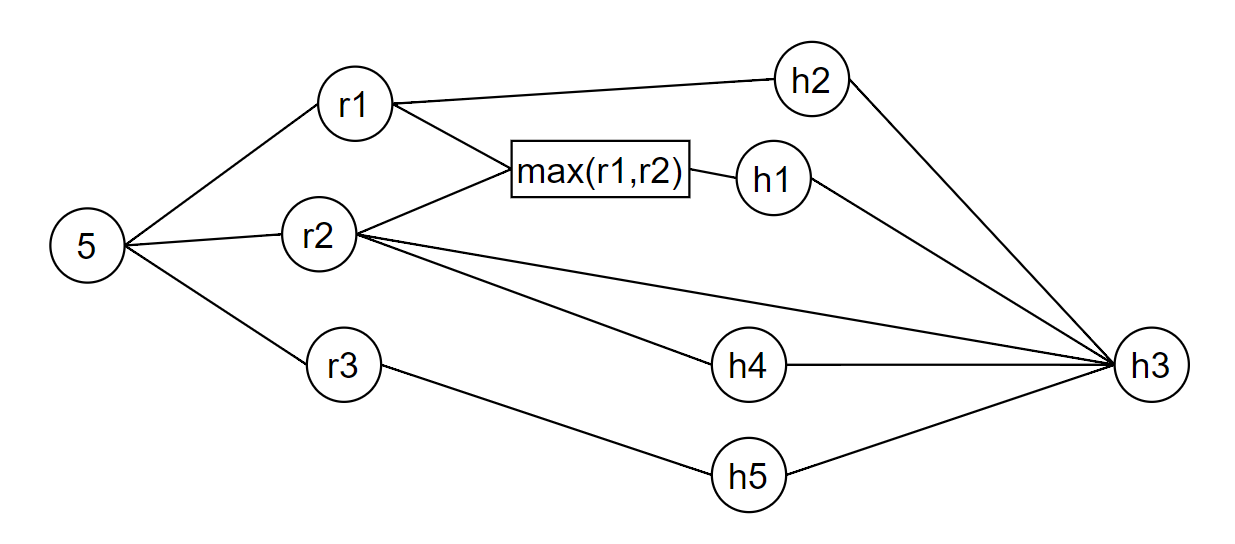
\includegraphics[width=8cm]{ConstraintGraph.png}
\centering
\end{figure}

\subsection{D - Backtracking search diagram}

\subsection{E - AC-3 diagram}

\begin{figure}[ht]
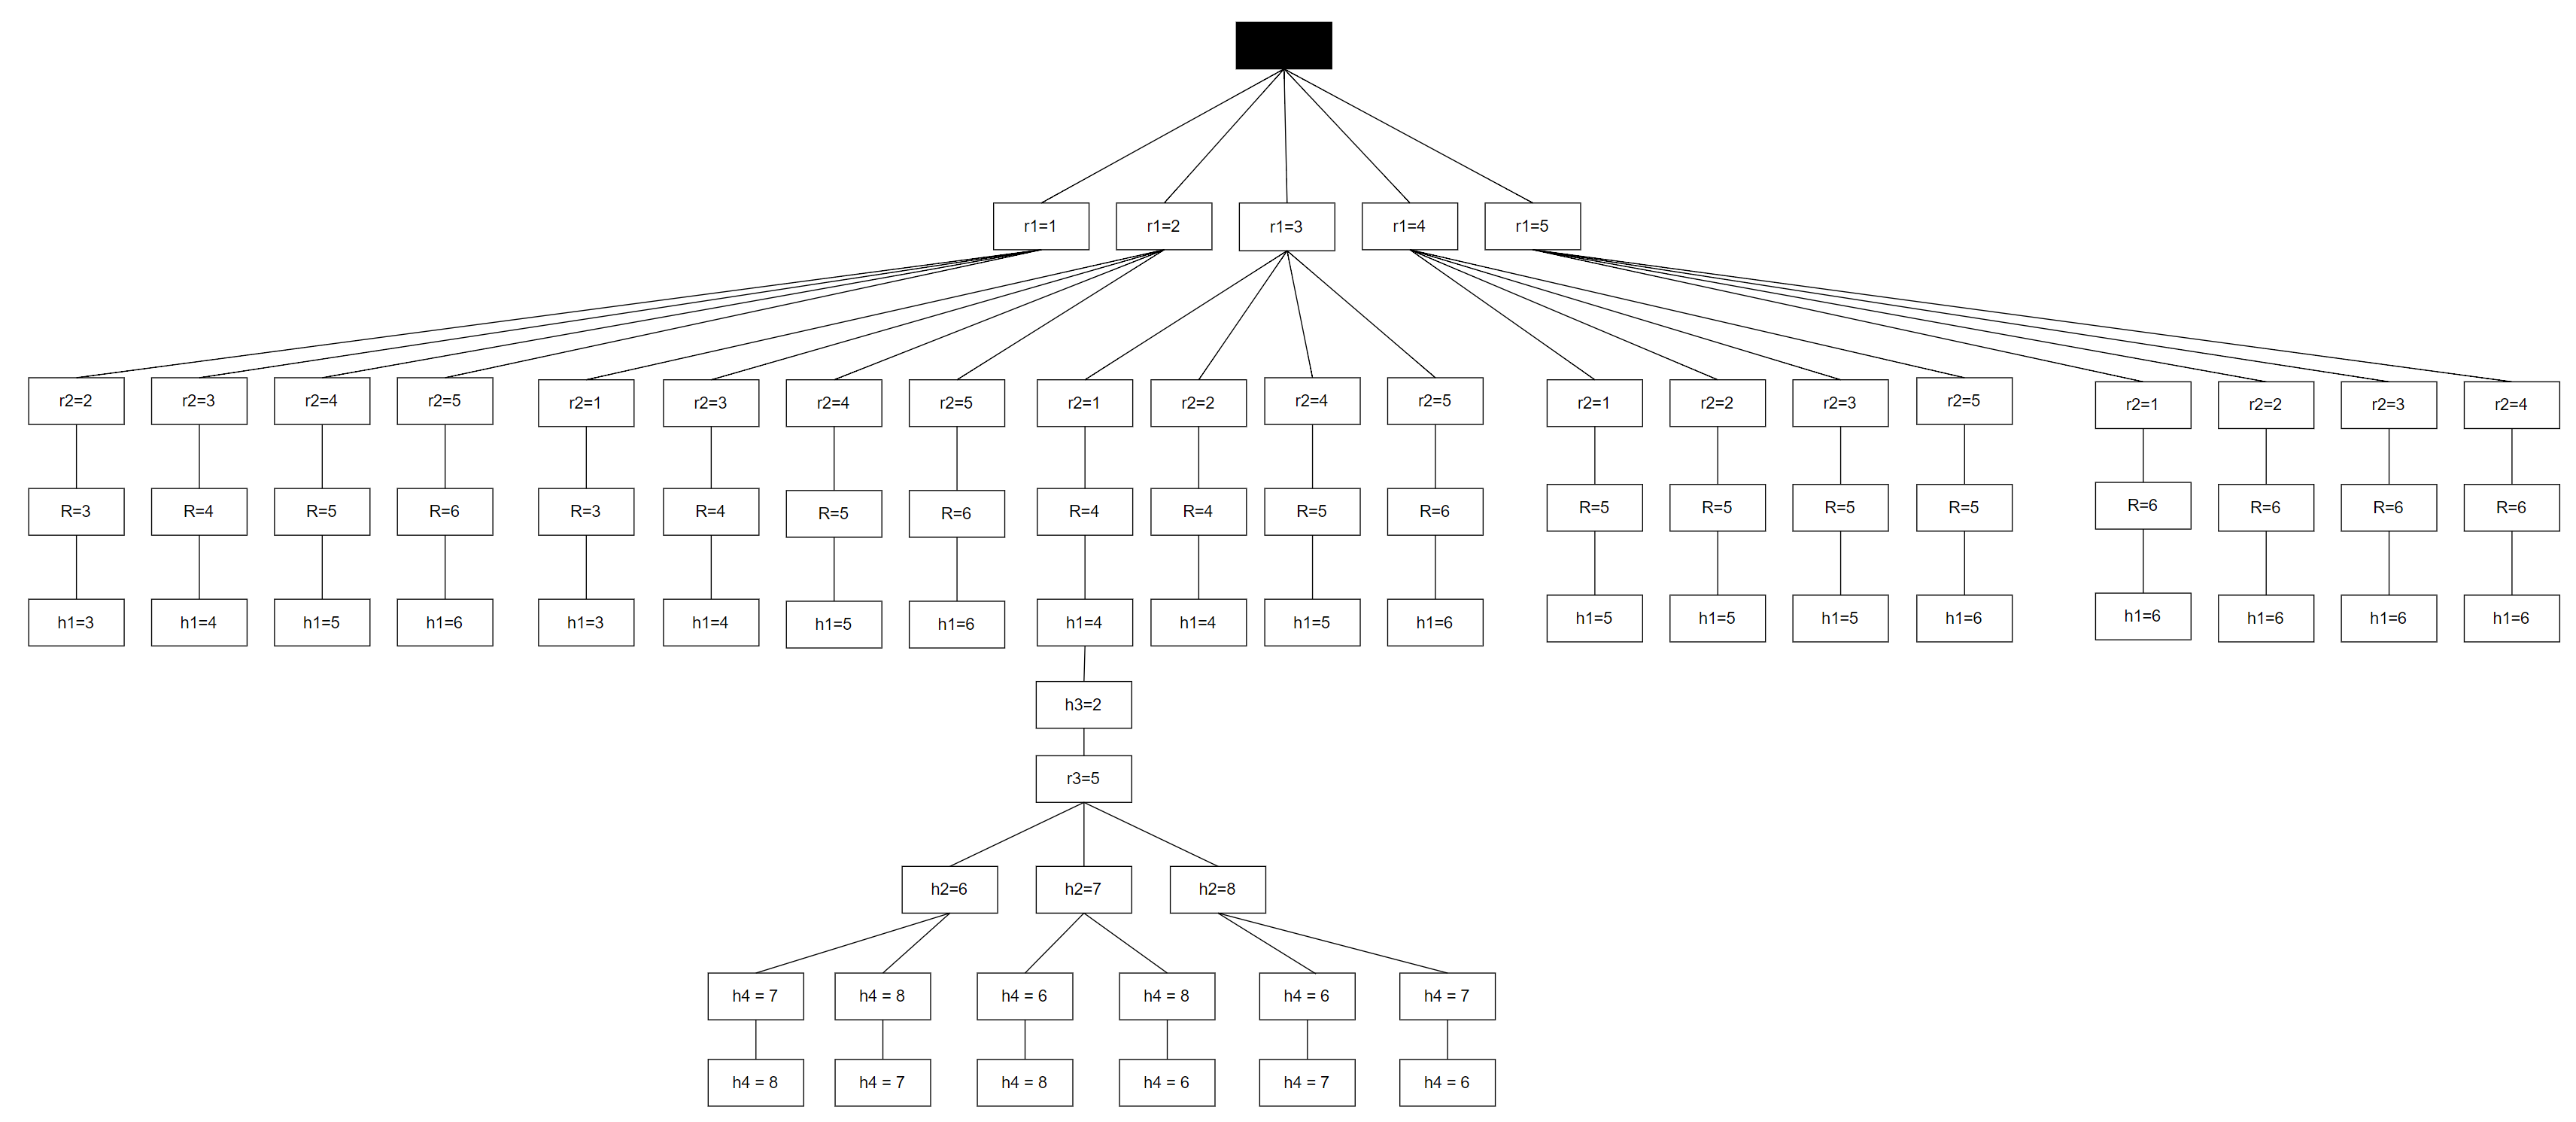
\includegraphics[width=18cm]{AC-3 Graph.png}
\centering
\end{figure}

\subsection{F - Pros and Cons}

AC-3 is far more efficient for this problem. For a similar problem in the future, I would choose AC-3 over backtracking search. 

\section{Part B - Search}

\subsection{A - Distance}

Manhattan distance would be an appropriate measure of distance, this is the sum of the horizontal and vertical distances which is applicable since drivers cannot move diagonally.

We can calculate it as:

For any two locations AB and CD where A and C represent the letter in the grid and B and D the number for each location, we can represent each letter with a number $0...16$, in ascending alphabetical order. $(x_1,y_1) = (A,B), (x_2,y_2) = (C,D)$.
E.g, the point C12 can be represented as (2,12)

The Manhattan distance can thus be represented as $$dist_M(l_1,l_2) = |x_1-x_2|+ |y_1-y_2|$$

\subsection{b - Driver heuristic}
$$ min\{dist_M(d_i, g)\}, \forall i \in \{1,2,3\}, \forall l \in goals$$

h1 driver: $$d_{h1} = min\{dist_M(d_i, r_1)\}, \forall i \in \{1,2,3\}$$
h2 driver: $$d_{h2} = min\{dist_M(d_i, r_2)\}, \forall i \in \{1,2,3\}$$
h3 driver: $$d_{h3} = min\{dist_M(d_i, r_3)\}, \forall i \in \{1,2,3\}$$

Using this heuristic we get 

h1 driver = H14
h2 driver = O1
h3 driver = P6

\subsection{c - A* Search}

\textbf{Driver 1} \newline
path start- r2 = N1 $\to$ M1 $\to $ M2 $\to$ M3 $\to$ M4 $\to$ L4 $\to$ K4 $\to$ J4 $\to$ I3 $\to$ I2 $\to$ I1 \newline
Nodes searched = N1, M1, M2, M3, N2, N3, M4, L4, K3, J4, K4, J4, I4, I3, I2 \newline
final frontier = I1, I3 \newline

path r2-h2

\textbf{Driver 2} \newline
path start - r3 = P7 $\to$ P8 $\to$ P9 $\to$ O10 $\to$ O11 $\to$ O12 $\to$ O13 $\to$ O14 $\to$ O15 $\to$ P16 \newline
Nodes searched: P7, P8, P9, O10, O11, O12, O13, O14, O15, P16 \newline
final frontier: O15,N16, P16



\textbf{Driver 3} \newline




\end{document}